%%%%%%%%%%%%%%%%%%%%%%%%%%%%%%%%%%%%%%%%%%%%%%%%%%%%%%%%%%%%%%
%%
%% Classes disponibles : 
%%	- times : utilisation de la police Times par défaut.
%%	- these, projthese, memoire, essai, rapport : pour 
%%		générer la page de garde en fonction du type document.
%%
%%%%%%%%%%%%%%%%%%%%%%%%%%%%%%%%%%%%%%%%%%%%%%%%%%%%%%%%%%%%%%%
\documentclass[12pt,times,these]{uqac}

%% Préciser l'emplacement du fichier contenant les acronymes.
\acrolistpath{assets/acro}

%% Toutes les images utilisées doivent se trouver dans le répertoire "figure".
\graphicspath{{figures/}}

%% Package pour activer le suivi des liens dans le PDF.
%% Il est possible de les identifier par une couleur différente du texte.
%% Par défaut, les liens ne sont pas différenciés du reste du texte.
\usepackage[hidelinks=true]{hyperref}

\begin{document}

% Titre du document
\title{Titre de la thèse du mémoire ou de l'essai}

% Auteur du document
\author{Prénom Nom}

%% Préciser le nom du programme
\programme{Informatique}

%% S’il y a lieu, 
%% indiquer le profil 
%% ou la concentration du programme
% \concentration{profil recherche}

%% Par défaut l'année courante est utilisée. 
%% Pour spéfier une autre année : 
% \degreeyear{2018}

\maketitle
		
%%%%%%%%%%%%%%%%%%%%%
%% Page préliminaires
%%%%%%%%%%%%%%%%%%%%%
\opening

\abstract{Lorem ipsum dolor sit amet, consectetur adipisicing elit, sed do eiusmod
tempor incididunt ut labore et dolore magna aliqua. Ut enim ad minim veniam,
quis nostrud exercitation ullamco laboris nisi ut aliquip ex ea commodo
consequat. Duis aute irure dolor in reprehenderit in voluptate velit esse
cillum dolore eu fugiat nulla pariatur. Excepteur sint occaecat cupidatat non
proident, sunt in culpa qui officia deserunt mollit anim id est laborum.}
\tableofcontents
\listoftables
\listoffigures
\listofacro
\begin{dedic}

Lorem ipsum dolor sit amet, consectetur adipisicing elit, sed do eiusmod
tempor incididunt ut labore et dolore magna aliqua. Ut enim ad minim veniam,
quis nostrud exercitation ullamco laboris nisi ut aliquip ex ea commodo
consequat. Duis aute irure dolor in reprehenderit in voluptate velit esse
cillum dolore eu fugiat nulla pariatur. Excepteur sint occaecat cupidatat non
proident, sunt in culpa qui officia deserunt mollit anim id est laborum.

\end{dedic}

\begin{ack}

Lorem ipsum dolor sit amet, consectetur adipisicing elit, sed do eiusmod
tempor incididunt ut labore et dolore magna aliqua. Ut enim ad minim veniam,
quis nostrud exercitation ullamco laboris nisi ut aliquip ex ea commodo
consequat. Duis aute irure dolor in reprehenderit in voluptate velit esse
cillum dolore eu fugiat nulla pariatur. Excepteur sint occaecat cupidatat non
proident, sunt in culpa qui officia deserunt mollit anim id est laborum.

\end{ack}

\begin{preface}

Lorem ipsum dolor sit amet, consectetur adipisicing elit, sed do eiusmod
tempor incididunt ut labore et dolore magna aliqua. Ut enim ad minim veniam,
quis nostrud exercitation ullamco laboris nisi ut aliquip ex ea commodo
consequat. Duis aute irure dolor in reprehenderit in voluptate velit esse
cillum dolore eu fugiat nulla pariatur. Excepteur sint occaecat cupidatat non
proident, sunt in culpa qui officia deserunt mollit anim id est laborum.

Lorem ipsum dolor sit amet, consectetur adipisicing elit, sed do eiusmod
tempor incididunt ut labore et dolore magna aliqua. Ut enim ad minim veniam,
quis nostrud exercitation ullamco laboris nisi ut aliquip ex ea commodo
consequat. Duis aute irure dolor in reprehenderit in voluptate velit esse
cillum dolore eu fugiat nulla pariatur. Excepteur sint occaecat cupidatat non
proident, sunt in culpa qui officia deserunt mollit anim id est laborum.

\end{preface}


%%%%%%%%%%%%%%%%%%%%%
%% Document principal
%%%%%%%%%%%%%%%%%%%%%
\maincontent

\introduction{Lorem ipsum dolor sit amet, consectetur adipisicing elit, sed do eiusmod
tempor incididunt ut labore et dolore magna aliqua. Ut enim ad minim veniam,
quis nostrud exercitation ullamco laboris nisi ut aliquip ex ea commodo
consequat. Duis aute irure dolor in reprehenderit in voluptate velit esse
cillum dolore eu fugiat nulla pariatur. Excepteur sint occaecat cupidatat non
proident, sunt in culpa qui officia deserunt mollit anim id est laborum.}
\chapter{Premier chapitre}
	
\section{sous-titre} 

Exemple d'utilisation d'un acronyme de trois lettres : \ac{TLA}.

\subsection{sous-titre} 

Lorem ipsum dolor sit amet, consectetur adipisicing elit, sed do eiusmod
tempor incididunt ut labore et dolore magna aliqua. Ut enim ad minim veniam,
quis nostrud exercitation ullamco laboris nisi ut aliquip ex ea commodo
consequat. Duis aute irure dolor in reprehenderit in voluptate velit esse
cillum dolore eu fugiat nulla pariatur. Excepteur sint occaecat cupidatat non
proident, sunt in culpa qui officia deserunt mollit anim id est laborum.

\subsection{sous-titre}   

Lorem ipsum dolor sit amet, consectetur adipisicing elit, sed do eiusmod
tempor incididunt ut labore et dolore magna aliqua. Ut enim ad minim veniam,
quis nostrud exercitation ullamco laboris nisi ut aliquip ex ea commodo
consequat. Duis aute irure dolor in reprehenderit in voluptate velit esse
cillum dolore eu fugiat nulla pariatur. Excepteur sint occaecat cupidatat non
proident, sunt in culpa qui officia deserunt mollit anim id est laborum.

Exemple de citation \cite{Ful83}.


\begin{figure}[H]
 \centering
 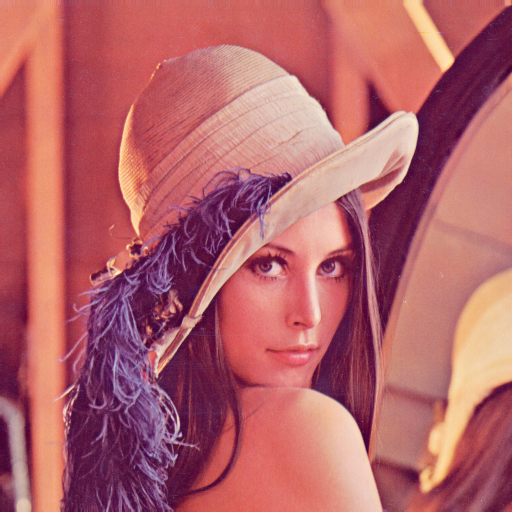
\includegraphics[width=7cm]{lenna.png}
 \caption{Titre de la figure}
 \label{fig:figure1}
\end{figure}

Lorem ipsum dolor sit amet, consectetur adipisicing elit, sed do eiusmod
tempor incididunt ut labore et dolore magna aliqua. Ut enim ad minim veniam,
quis nostrud exercitation ullamco laboris nisi ut aliquip ex ea commodo
consequat. Duis aute irure dolor in reprehenderit in voluptate velit esse
cillum dolore eu fugiat nulla pariatur. Excepteur sint occaecat cupidatat non
proident, sunt in culpa qui officia deserunt mollit anim id est laborum.

\section{sous-titre}   

Lorem ipsum dolor sit amet, consectetur adipisicing elit, sed do eiusmod
tempor incididunt ut labore et dolore magna aliqua. Ut enim ad minim veniam,
quis nostrud exercitation ullamco laboris nisi ut aliquip ex ea commodo
consequat. Duis aute irure dolor in reprehenderit in voluptate velit esse
cillum dolore eu fugiat nulla pariatur. Excepteur sint occaecat cupidatat non
proident, sunt in culpa qui officia deserunt mollit anim id est laborum.

Lorem ipsum dolor sit amet, consectetur adipisicing elit, sed do eiusmod
tempor incididunt ut labore et dolore magna aliqua. Ut enim ad minim veniam,
quis nostrud exercitation ullamco laboris nisi ut aliquip ex ea commodo
consequat.

\chapter{second chapitre}

\section{exemples avancés}

\subsection{équations}

\begin{equation}
  \label{eq:eq_1}
  E=mc^2
\end{equation}

Il est possible de référencer l'Équation \ref{eq:eq_1} dans le texte.

\subsection{théorèmes et preuves}

\begin{theorem}
  \label{theo:theo_1}
  Let $f$ be a function whose derivative exists in every point, then $f$ is
  a continuous function.
\end{theorem}

\begin{theorem}[Pythagorean theorem]
  \label{theo:theo_2}
  This is a theorema about right triangles and can be summarised in the next
  equation
  \[ x^2 + y^2 = z^2 \]
\end{theorem}

\begin{corollary}
  \label{coro:coro_1}
  There's no right rectangle whose sides measure 3cm, 4cm, and 6cm.
\end{corollary}

\begin{lemma}
  \label{lem:lem_1}
  Given two line segments whose lengths are $a$ and $b$ respectively there
  is a real number $r$ such that $b=ra$.
\end{lemma}

\begin{definition}[Fibration]
  \label{def:def_1}
  A fibration is a mapping between two topological spaces that has the homotopy lifting property for every space $X$.
\end{definition}

\begin{proof}
  \label{proof:proof_1}
  To prove it by contradiction try and assume that the statement is false,
  proceed from there and at some point you will arrive to a contradiction.
\end{proof}

Vous pouvez ensuite référencer les Théorèmes \ref{theo:theo_1} et \ref{theo:theo_2}, ainsi que le Corollaire \ref{coro:coro_1} et le Lemme \ref{lem:lem_1} dans votre texte. De plus, la Définition \ref{def:def_1} et la Démonstration \ref{proof:proof_1} peuvent également être référencées dans le texte.

\subsection{algorithmes}

\begin{algorithm}[H]
  \KwData{input}
  \KwResult{output}
  initialization\;
   \While{predicat}{
    instructions\;
    \eIf{condition}{
     instructions1\;
     instructions2\;
     }{
     instructions3\;
    }
   }
  \caption{Titre de l'algorithme.}
  \label{algo:algo_1}
\end{algorithm}

L'algorithme \ref{algo:algo_1} peut ensuite être référencé dans le texte.

\chapter{troisième chapitre}

\section{Informatique}

Vous pouvez inclure du code de la manière suivante :

\begin{minted}[frame=single,framesep=2mm,baselinestretch=1,fontsize=\footnotesize,linenos]{cpp}
{
  #include <iostream>

  int main() {
      std::cout << "Hello World!";
      return 0;
  }
}
\end{minted}

\section{Chimie}

Vous pouvez inclure des formules chimiques de la manière suivante :

\begin{figure}[H]
  \centering
  \chemfig{-[:30](=[:90]O)-[:-30]OH}
  \caption{La formule de l'Éthanol.}
  \label{fig:ethanol}
\end{figure}

\noindent La formule de l'Éthanol est représentée en Figure \ref{fig:ethanol}.

\section{Ingénierie}

Vous pouvez inclure des schémas électriques de la manière suivante :

\begin{figure}[H]
  \centering
  \begin{circuitikz}[american voltages]
    \draw
      (0,0) to [short, *-] (6,0)
      to [V, l_=$\mathrm{j}{\omega}_m \underline{\psi}^s_R$] (6,2)
      to [R, l_=$R_R$] (6,4)
      to [short, i_=$\underline{i}^s_R$] (5,4)

      (0,0) to [open, v^>=$\underline{u}^s_s$] (0,4)
      to [short, *- ,i=$\underline{i}^s_s$] (1,4)
      to [R, l=$R_s$] (3,4)
      to [L, l=$L_{\sigma}$] (5,4)
      to [short, i_=$\underline{i}^s_M$] (5,3)
      to [L, l_=$L_M$] (5,0);
  \end{circuitikz}
  \caption{Exemple d'un schéma électriques.}
  \label{fig:elec}
\end{figure}

\noindent La Figure \ref{fig:elec} montre un exemple de schéma électriques.

\section{Physique}

Vous pouvez inclure des diagrammes de Feynman de la manière suivante :

\begin{figure}[H]
  \centering
  \feynmandiagram [small, horizontal=a to t1] {
    a [particle=\(\pi^{0}\)] -- [scalar] t1 -- t2 -- t3 -- t1,
    t2 -- [photon] p1 [particle=\(\gamma\)],
    t3 -- [photon] p2 [particle=\(\gamma\)],
  };
  \caption{Exemple d'un diagramme de Feynman.}
  \label{fig:feynman}
\end{figure}

\noindent La Figure \ref{fig:feynman} montre l'exemple d'un diagramme de Feynman.

\begin{conclusion}

Lorem ipsum dolor sit amet, consectetur adipisicing elit, sed do eiusmod
tempor incididunt ut labore et dolore magna aliqua. Ut enim ad minim veniam,
quis nostrud exercitation ullamco laboris nisi ut aliquip ex ea commodo
consequat. Duis aute irure dolor in reprehenderit in voluptate velit esse
cillum dolore eu fugiat nulla pariatur. Excepteur sint occaecat cupidatat non
proident, sunt in culpa qui officia deserunt mollit anim id est laborum.

\end{conclusion}

%%%%%%%%$%%%%
%% Références
%%%%%%%%%%%%%

\bibliographystyle{apa-uqac}
\bibliography{references}

%%%%%%%%%%%
%% Annexes
%%%%%%%%%%%
\appendix

\chapter{Première Annexe}

Lorem ipsum dolor sit amet, consectetur adipisicing elit, sed do eiusmod
tempor incididunt ut labore et dolore magna aliqua. Ut enim ad minim veniam,
quis nostrud exercitation ullamco laboris nisi ut aliquip ex ea commodo
consequat. Duis aute irure dolor in reprehenderit in voluptate velit esse
cillum dolore eu fugiat nulla pariatur. Excepteur sint occaecat cupidatat non
proident, sunt in culpa qui officia deserunt mollit anim id est laborum.

\end{document}
